\documentclass[11pt]{article}

\usepackage[margin=1in]{geometry}
\usepackage{times}
\usepackage[T1]{fontenc}
\usepackage[utf8]{inputenc}
\usepackage{microtype}
\usepackage{amsmath,amssymb}
\usepackage{booktabs}
\usepackage{graphicx}
\usepackage[font=small,labelfont=bf]{caption}
\usepackage{hyperref}
\usepackage[numbers]{natbib}

% Shared notation for the benchmark paper.
\newcommand{\AUPRC}{AUPRC}
\newcommand{\AUROC}{AUROC}

\hypersetup{hidelinks}
\setlength{\textfloatsep}{10pt plus 2pt minus 2pt}
\setlength{\floatsep}{8pt plus 2pt minus 2pt}
\setlength{\intextsep}{8pt plus 2pt minus 2pt}

\title{Synthetic Cold Splits Are Not Enough: Distribution-Shift Benchmarking for Drug-Target Interaction Prediction}
\author{Anonymous Authors}
\date{}

\begin{document}
\maketitle

\begin{abstract}
Drug-target interaction (DTI) papers often use synthetic cold-start splits as proxies for generalization, but it remains unclear whether conclusions drawn from these splits transfer to real distribution shifts. We present a benchmark-first study showing that model rankings are highly sensitive to how the shift is defined. Using a compact panel consisting of a plain base encoder, a retrieval-augmented model (\texttt{RAICD}), and a functional target-memory variant (\texttt{FTM sparse}), we first build a 3-seed synthetic reference panel on \texttt{BindingDB\_Kd}. Even within this single dataset, rankings are heterogeneous: \texttt{RAICD} improves over the base model on \texttt{blind\_start}, loses on \texttt{unseen\_drug}, and \texttt{FTM sparse} is strongest on synthetic \texttt{unseen\_target}. We then evaluate the same panel on a real temporal/provenance benchmark, \texttt{BindingDB\_patent / patent\_temporal}, where the internal-panel ranking reverses. Over 3 seeds, the plain base model achieves $0.7772 \pm 0.0086$ \AUPRC{}, outperforming both \texttt{RAICD} ($0.7692 \pm 0.0018$) and \texttt{FTM sparse} ($0.7721 \pm 0.0025$). When we expand the model panel with recent pooled-LM baselines, \texttt{DTI-LM} becomes the strongest patent model at $0.7825 \pm 0.0078$ \AUPRC{}, and the same winner is preserved under an earlier alternative patent cutoff. Paired bootstrap intervals confirm the sign of the key \AUPRC{} deltas. A year-band and overlap-bucket diagnosis further shows that temporal OOD is structured rather than monolithic. Matched 3-seed support from \texttt{BindingDB\_Ki} and \texttt{DAVIS} indicates that synthetic \texttt{unseen\_target} gains are not reliably portable, and we package the split manifests and evaluator as reusable benchmark resources. Within the studied model panel and benchmarks, these results show that synthetic cold splits and real OOD shifts are not interchangeable evaluation settings for DTI.

\end{abstract}

\section{Introduction}

Predicting drug-target interactions for unseen molecules or proteins is a central goal in computational drug discovery. Because truly prospective evaluation is difficult and expensive, many recent studies report held-out drug, target, or blind splits on datasets derived from BindingDB or DAVIS as proxies for inductive generalization \citep{liu2007bindingdb,davis2011kinase,ahmed2024dtilm,luo2024druglamp,ouyang2024pmmr,liu2025spdti,yu2025gsdti,zhao2025coldstartcpi}. These protocols are useful, but they also encourage a strong implicit assumption: if a method performs well on one cold-start split, then it is broadly robust to the kinds of shift encountered in deployment.

That assumption is weaker than it appears. Different split definitions remove different forms of overlap, and they may favor different inductive biases. A retrieval mechanism can help when nearby support examples remain informative, yet become much less useful when the promoted benchmark introduces temporal, provenance, or assay changes that are not captured by synthetic exclusion rules. Likewise, a target-memory mechanism may appear beneficial on one synthetic regime while failing to transfer across datasets or assay families. If these ranking changes occur in practice, benchmark design is not a technical footnote. It becomes part of the scientific claim.

This paper studies that question directly. Rather than proposing another universal architecture, we ask whether the ranking of a compact DTI model panel is preserved across synthetic cold-start regimes and real distribution shifts. Our starting point is a synthetic reference panel on \texttt{BindingDB\_Kd}, where we compare three representative systems: a plain base encoder, a retrieval-augmented model (\texttt{RAICD}), and a functional target-memory model (\texttt{FTM sparse}). Even here, rankings are already heterogeneous: \texttt{RAICD} improves on \texttt{blind\_start}, loses on \texttt{unseen\_drug}, and \texttt{FTM sparse} is strongest on synthetic \texttt{unseen\_target}.

We then contrast this synthetic picture with a real temporal/provenance benchmark built from the BindingDB patent split (\texttt{patent\_temporal}), using matched 3-seed evaluation. The result is a clear ranking reversal. On synthetic \texttt{blind\_start}, retrieval is beneficial; on patent temporal shift, the plain base model is best, outperforming both \texttt{RAICD} and \texttt{FTM sparse}. Paired bootstrap confidence intervals support both parts of this contrast: the synthetic \texttt{blind\_start} \AUPRC{} delta for \texttt{RAICD - base} remains positive, while the patent-temporal deltas for both \texttt{RAICD - base} and \texttt{FTM - base} remain negative.

To move beyond leaderboard-style reporting, we also diagnose the promoted temporal benchmark by year and overlap bucket. This analysis shows that temporal OOD is not simply ``harder cold-start.'' Instead, the gap is concentrated in specific year bands and overlap regimes, which helps explain why a method that looks strong under one split can lose under another. We further include \texttt{BindingDB\_Ki} and \texttt{DAVIS} as supporting real-OOD screens, showing that the synthetic \texttt{unseen\_target} advantage of \texttt{FTM sparse} does not transfer reliably outside the original benchmark. Recent molecular benchmark studies have made analogous arguments about OOD sensitivity in adjacent tasks \citep{ektefaie2024generalizability,shen2025ddiben,delafuente2025inductive}; our contribution is to show the same issue concretely in DTI.

Our contributions are fourfold. First, we construct a 3-seed synthetic reference panel showing that even standard cold-start evaluation is regime-dependent. Second, we establish a 3-seed real-OOD benchmark on \texttt{BindingDB\_patent} and show a ranking reversal relative to synthetic \texttt{blind\_start}. Third, we provide year-band and overlap-bucket analyses that connect the ranking change to measurable shift axes. Fourth, we show through supporting benchmarks that method gains observed on synthetic \texttt{unseen\_target} are not robust enough to serve as a universal claim.

\section{Related Work}

\paragraph{Synthetic cold-start evaluation in DTI.}
Machine-learning models for DTI and affinity prediction are commonly evaluated on BindingDB- and DAVIS-derived random, cold-drug, cold-target, or blind splits \citep{liu2007bindingdb,davis2011kinase,ahmed2024dtilm,luo2024druglamp,ouyang2024pmmr,liu2025spdti,yu2025gsdti,zhao2025coldstartcpi}. These protocols are useful for controlled comparison, but they eliminate different forms of chemical, protein, and pair overlap and therefore do not represent a single validation setting. For this reason, results obtained on one synthetic split should not automatically be interpreted as evidence of general robustness.

\paragraph{Validation design in chemoinformatics.}
More broadly in chemoinformatics, validation design and test-set construction are known to influence apparent model performance. Reanalysis of large bioactivity benchmarks, increasingly challenging potency-prediction partitions, and transfer-learning studies for binary drug--target interactions have all shown that the relative standing of deep and classical models can change materially when the evaluation setting changes \citep{robinson2020validating,rodriguezperez2021evaluation,tanoori2021binding}. Our study follows this validation-oriented tradition by asking how split semantics alter conclusions in a DTI setting built around widely used BindingDB and DAVIS resources.

\paragraph{Benchmark and resource studies under distribution shift.}
Recent benchmark studies in molecular machine learning and related biomedical prediction problems have shown that scaffold, temporal, and domain-shifted evaluation can change model ranking and alter the practical interpretation of benchmark results \citep{ektefaie2024generalizability,shen2025ddiben,delafuente2025inductive}. This literature has shifted attention from purely i.i.d.\ comparison toward reusable benchmark resources that expose how conclusions depend on data partitioning. Our work extends that perspective to DTI by coupling multiple benchmark families with exported split manifests and a standalone evaluator.

\paragraph{Positioning.}
Prior DTI papers typically optimize performance within one benchmark design. In contrast, our contribution is a reproducible case study of ranking stability across synthetic cold-start and temporal/provenance benchmarks, together with overlap-sensitive robustness analyses and reusable evaluation resources. The emphasis is therefore on validation methodology and benchmark semantics rather than on proposing a new predictive architecture.

\section{Benchmark Setup}

Our goal is to test whether a compact DTI model panel preserves its ranking across synthetic cold-start regimes and real distribution shifts. The panel contains three models: \texttt{base}, a plain encoder that serves as the reference system; \texttt{RAICD}, a retrieval-augmented model that aggregates support from similar seen entities; and \texttt{FTM sparse}, a functional target-memory model designed to improve target-cold generalization. We intentionally keep the panel small so that benchmark effects are not obscured by a large architecture zoo.

We evaluate this panel on two benchmark groups. The first is a synthetic reference panel based on \texttt{BindingDB\_Kd}, with three split definitions: \texttt{unseen\_drug}, \texttt{blind\_start}, and \texttt{unseen\_target}. The second is a real-OOD screening panel. Our primary real-OOD benchmark is the BindingDB patent split (\texttt{patent\_temporal}), which uses a year-based temporal partition and is evaluated over three seeds. We also include \texttt{BindingDB\_Ki / unseen\_target} and \texttt{DAVIS / unseen\_target} as supporting screens that test whether the synthetic \texttt{unseen\_target} gain of \texttt{FTM sparse} transfers across assay and dataset shifts. Table~\ref{tab:taxonomy} summarizes the shift taxonomy and split statistics.

\begin{table}[t]
  \centering
  \scriptsize
  \caption{Benchmark taxonomy and seed0 split statistics. Test prevalence differs substantially across benchmark families, so \AUPRC{} should be compared within benchmark rather than across rows.}
  \label{tab:taxonomy}
  \setlength{\tabcolsep}{4pt}
  \resizebox{\linewidth}{!}{
  \begin{tabular}{@{}llrrr@{}}
    \toprule
    Benchmark & Shift family & Synth.? & Test rows & Pos. rate \\
    \midrule
    \texttt{Kd / unseen\_drug} & drug-cold & yes & 12,744 & 0.1966 \\
    \texttt{Kd / blind\_start} & drug+target-cold & yes & 2,821 & 0.2031 \\
    \texttt{Kd / unseen\_target} & target-cold & yes & 12,052 & 0.2239 \\
    \texttt{patent / patent\_temporal} & temporal+source & no & 49,028 & 0.5745 \\
    \texttt{Ki / unseen\_target} & assay+target-cold & mixed & 70,380 & 0.4652 \\
    \texttt{DAVIS / unseen\_target} & dataset+target-cold & mixed & 5,168 & 0.0615 \\
    \bottomrule
  \end{tabular}}
\end{table}


We report \AUPRC{} as the primary metric and \AUROC{} as a secondary metric. \AUPRC{} is emphasized because class balance and ranking behavior are central to the benchmark claims in this paper. For the synthetic reference panel and the promoted patent benchmark, we report matched three-seed results. For \texttt{BindingDB\_Ki} and \texttt{DAVIS}, we report seed0 support only and treat these as supporting rather than headline evidence. We further add paired bootstrap uncertainty support for the key ranking reversals: \texttt{RAICD} versus \texttt{base} on synthetic \texttt{blind\_start}, and \texttt{base} versus \texttt{RAICD} or \texttt{FTM} on patent temporal.

The patent benchmark requires several setup choices that are documented explicitly. We use a local year-based split of \texttt{BindingDB\_patent}, with training years before the validation year, a held-out validation year, and a later temporal test set. Because this benchmark also changes provenance and assay composition, we describe it as temporal/provenance OOD rather than pure time shift. We also use a patent-specific affinity conversion rather than reusing the standard \texttt{pKd} transform, because the patent benchmark stores affinities in a different log-scale convention. BindingDB-derived panels are anchored in the BindingDB resource \citep{liu2007bindingdb}, while DAVIS provides an external kinase-focused support benchmark \citep{davis2011kinase}.

Finally, for diagnostic analysis, we use the saved overlap score from each test prediction to compute overlap buckets that summarize how strongly each test example resembles the training support. We report benchmark taxonomy and split statistics, including test-set size and prevalence, so that \AUPRC{} is interpreted within benchmark rather than across benchmark families.

\section{Results}

\subsection{Synthetic cold splits are already regime-dependent}

We begin with the \texttt{BindingDB\_Kd} synthetic reference panel. Table~\ref{tab:main-results} shows the main pattern: even within a single dataset, model rankings are not stable across split definitions. On \texttt{unseen\_drug}, \texttt{HyperPCM} is strongest by mean \AUPRC{}, reaching $0.5694 \pm 0.0473$ versus $0.5509 \pm 0.0900$ for \texttt{base} and $0.5004 \pm 0.0341$ for \texttt{DTI-LM}. On \texttt{blind\_start}, \texttt{HyperPCM} again has the highest mean \AUPRC{} at $0.3828 \pm 0.1024$, but the margin over \texttt{base} is much smaller and the variance is larger. On \texttt{unseen\_target}, the pattern changes again: \texttt{base} is strongest by mean \AUPRC{} at $0.5224 \pm 0.0602$, while \texttt{DTI-LM} is slightly lower on \AUPRC{} but higher on mean \AUROC{}.

\begin{table}[t]
  \centering
  \scriptsize
  \caption{Synthetic reference panel and promoted real-OOD benchmark. Values are mean $\pm$ std over seeds. Best mean \AUPRC{} in each row is bold.}
  \label{tab:main-results}
  \setlength{\tabcolsep}{3.5pt}
  \resizebox{\linewidth}{!}{
  \begin{tabular}{@{}llcccc@{}}
    \toprule
    Benchmark & Seeds & base (\AUPRC{}/\AUROC{}) & RAICD (\AUPRC{}/\AUROC{}) & FTM sparse (\AUPRC{}/\AUROC{}) & Winner \\
    \midrule
    \texttt{BindingDB\_Kd / unseen\_drug} & 3 &
    \textbf{0.5509 $\pm$ 0.0900 / 0.7794 $\pm$ 0.0534} &
    0.5228 $\pm$ 0.0828 / 0.7803 $\pm$ 0.0506 &
    -- &
    base \\
    \texttt{BindingDB\_Kd / blind\_start} & 3 &
    0.3737 $\pm$ 0.0229 / 0.6778 $\pm$ 0.0151 &
    \textbf{0.4024 $\pm$ 0.0508 / 0.6844 $\pm$ 0.0145} &
    -- &
    RAICD \\
    \texttt{BindingDB\_Kd / unseen\_target} & 3 &
    0.5224 $\pm$ 0.0602 / 0.7741 $\pm$ 0.0161 &
    -- &
    \textbf{0.5439 $\pm$ 0.0791 / 0.7848 $\pm$ 0.0204} &
    FTM \\
    \texttt{BindingDB\_patent / patent\_temporal} & 3 &
    \textbf{0.7772 $\pm$ 0.0086 / 0.7223 $\pm$ 0.0109} &
    0.7692 $\pm$ 0.0018 / 0.7032 $\pm$ 0.0010 &
    0.7721 $\pm$ 0.0025 / 0.7059 $\pm$ 0.0037 &
    base \\
    \bottomrule
  \end{tabular}}
\end{table}


These results matter because they show that ``synthetic cold-start DTI'' is already not a single evaluation condition. Even after replacing internal probes with external literature baselines, different synthetic regimes still reward different model families, so it is unsafe to generalize from one split to another without explicit evidence.

\subsection{Real temporal shift favors a different strong baseline}

We next evaluate the same external panel on \texttt{BindingDB\_patent / patent\_temporal}, our primary real-OOD benchmark. Over three seeds, \texttt{DTI-LM} is the strongest model by mean \AUPRC{}, reaching $0.7825 \pm 0.0078$, compared with $0.7772 \pm 0.0086$ for \texttt{base} and $0.7753 \pm 0.0050$ for \texttt{HyperPCM}. Figure~\ref{fig:delta-summary} compresses the main benchmark story into within-benchmark \AUPRC{} deltas relative to \texttt{base}: synthetic cold splits favor different systems, while the promoted temporal benchmark favors \texttt{DTI-LM}. This temporal advantage is also supported by paired bootstrap: \texttt{DTI-LM - base} $= +0.0054$ with 95\% CI $[+0.0028, +0.0079]$.

\begin{figure}[t]
  \centering
  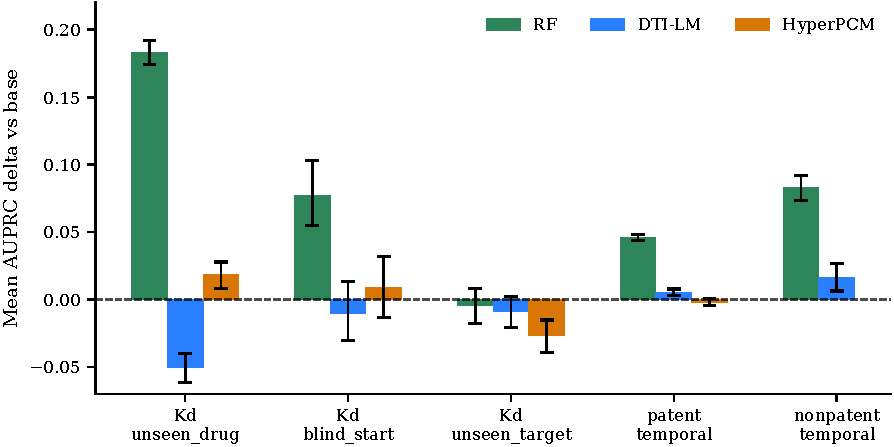
\includegraphics[width=\linewidth]{figures/benchmark_delta_summary.pdf}
  \caption{Mean \AUPRC{} delta relative to \texttt{base} within each benchmark under the external replacement panel. Error bars show paired bootstrap 95\% intervals where available. The synthetic axes and the promoted patent benchmark favor different systems.}
  \label{fig:delta-summary}
\end{figure}

This is the central winner change in the revised paper. The synthetic panel does not produce a single best model, but the promoted temporal benchmark clearly favors \texttt{DTI-LM} by mean \AUPRC{}. The alternative-cutoff benchmark tells the same story over matched three-seed evaluation: on \texttt{patent\_temporal\_v2017}, \texttt{DTI-LM} reaches $0.7134 \pm 0.0027 / 0.6754 \pm 0.0039$, versus $0.7044 \pm 0.0058 / 0.6624 \pm 0.0079$ for \texttt{base}. The broader lesson is therefore not that one external baseline wins everywhere, but that both benchmark axis and model family change the apparent ranking.

\subsection{Temporal shift is structured across year bands and overlap levels}

To help explain why the temporal benchmark changes the ranking, we analyze the patent results by year and by overlap bucket. Table~\ref{tab:patent-diagnosis-compact} makes the primary \AUPRC{} slices explicit, while Figure~\ref{fig:patent-diagnosis} visualizes the same structure. In the large 2019 slice, \texttt{DTI-LM} is strongest by mean \AUPRC{} ($0.7734$), with \texttt{base} ($0.7626$) and \texttt{HyperPCM} ($0.7637$) close behind. In 2020, however, the ordering flips: \texttt{base} reaches $0.8715 / 0.8135$, while \texttt{DTI-LM} and \texttt{HyperPCM} drop to $0.8545 / 0.7951$ and $0.8526 / 0.7938$, respectively. The 2021 slice is small, but again strongly favors \texttt{base}.

The overlap-bucket analysis reveals another useful pattern. In the lowest-overlap bucket, \texttt{DTI-LM} is strongest by mean \AUPRC{} ($0.6353$), while \texttt{HyperPCM} is close behind. In the middle-overlap bucket, \texttt{HyperPCM} takes a small lead on \AUPRC{} ($0.7513$) over \texttt{DTI-LM} ($0.7489$) and \texttt{base} ($0.7218$). In the highest-overlap bucket, the ordering flips again and \texttt{base} dominates on both \AUPRC{} and \AUROC{}. Together, these results are consistent with the view that temporal OOD is not just a colder version of synthetic cold-start. Instead, it changes which subpopulations dominate the aggregate result, and therefore changes the model ranking.

\begin{table}[t]
  \centering
  \scriptsize
  \caption{Compact \AUPRC{} summary behind the patent diagnosis under the external replacement panel. Values are mean $\pm$ seed std over the matched 3-seed runs. The tiny 2021 slice is pooled into the \texttt{2020--2021} stratum to avoid over-interpreting a 72-example cell.}
  \label{tab:patent-diagnosis-compact}
  \setlength{\tabcolsep}{3.5pt}
  \resizebox{\linewidth}{!}{
  \begin{tabular}{@{}llcccc@{}}
    \toprule
    Slice type & Slice & Count & base & DTI-LM & HyperPCM \\
    \midrule
    Year & 2019 & 42,009 & 0.7626 $\pm$ 0.0098 & \textbf{0.7734 $\pm$ 0.0071} & 0.7637 $\pm$ 0.0049 \\
    Year & 2020--2021 & 7,019 & \textbf{0.8716 $\pm$ 0.0121} & 0.8533 $\pm$ 0.0100 & 0.8516 $\pm$ 0.0139 \\
    Overlap bucket & 0 ($0.000$--$0.531$) & 16,341 & 0.5551 $\pm$ 0.0190 & \textbf{0.6353 $\pm$ 0.0175} & 0.6147 $\pm$ 0.0208 \\
    Overlap bucket & 1 ($0.531$--$0.710$) & 16,342 & 0.7218 $\pm$ 0.0167 & 0.7489 $\pm$ 0.0094 & \textbf{0.7513 $\pm$ 0.0060} \\
    Overlap bucket & 2 ($0.710$--$0.989$) & 16,345 & \textbf{0.9237 $\pm$ 0.0030} & 0.8866 $\pm$ 0.0097 & 0.8767 $\pm$ 0.0042 \\
    \bottomrule
  \end{tabular}}
\end{table}


\begin{figure}[t]
  \centering
  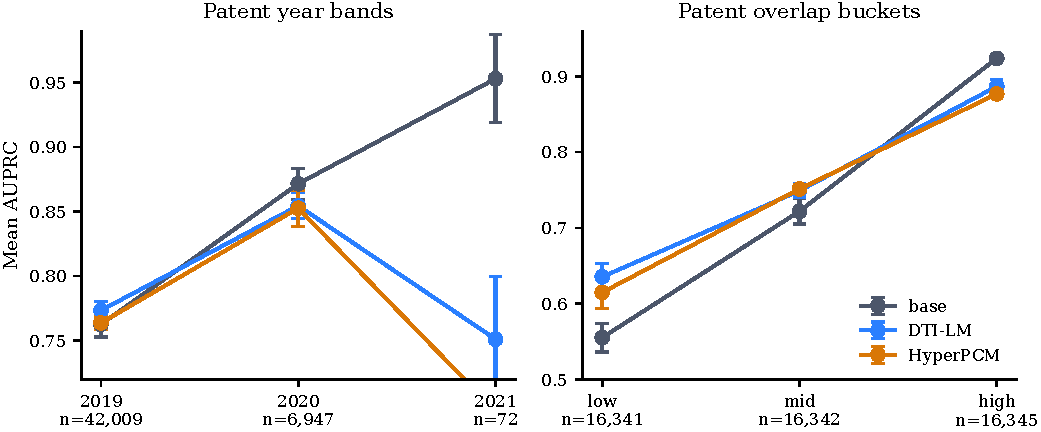
\includegraphics[width=\linewidth]{figures/patent_shift_diagnosis.pdf}
  \caption{Patent temporal diagnosis in terms of mean \AUPRC{} under the external replacement panel. Left: year-band slices. Right: test-set overlap buckets computed from the saved overlap score. The aggregate \texttt{DTI-LM} advantage is concentrated in the 2019 and lower-overlap strata, while \texttt{base} dominates the 2020 and highest-overlap slices.}
  \label{fig:patent-diagnosis}
\end{figure}

\subsection{Supporting target-cold OOD benchmarks still favor the plain base model}

We treat \texttt{BindingDB\_Ki / unseen\_target} and \texttt{DAVIS / unseen\_target} as supporting real-OOD benchmarks rather than primary headline axes. Under matched three-seed evaluation, neither promoted external baseline overturns the support-panel story. On \texttt{BindingDB\_Ki}, \texttt{base} reaches $0.6934 \pm 0.0257 / 0.7192 \pm 0.0068$, compared with $0.6648 \pm 0.0177 / 0.6936 \pm 0.0044$ for \texttt{DTI-LM} and $0.6515 \pm 0.0301 / 0.6757 \pm 0.0211$ for \texttt{HyperPCM}. On \texttt{DAVIS}, \texttt{base} reaches $0.4097 \pm 0.0275 / 0.8613 \pm 0.0153$, compared with $0.4090 \pm 0.0570 / 0.8718 \pm 0.0152$ for \texttt{DTI-LM} and $0.3840 \pm 0.0269 / 0.8610 \pm 0.0245$ for \texttt{HyperPCM}.

The \texttt{DAVIS} result is the closest supporting-panel case: \texttt{DTI-LM} is effectively tied with \texttt{base} on mean \AUPRC{} and slightly higher on mean \AUROC{}, but it still does not create a clean winner change of the kind seen on the promoted patent benchmark. \texttt{BindingDB\_Ki} is more decisive, with \texttt{base} ahead of both external baselines on both metrics. These auxiliary results are therefore consistent with the main claim of the paper, but they do not carry the same argumentative weight as the patent benchmark because they do not add a cleaner ranking-reversal axis than temporal/provenance shift.

\section{Discussion}

The main message of this study is that, within the studied expanded panel, DTI evaluation is benchmark-sensitive in a way that current reporting practice often obscures. A synthetic split can still be useful, but it should not be treated as a universal proxy for real OOD generalization. Once the panel includes pooled-LM baselines, a graph-family probe, and a learner-control classical baseline on the same handcrafted inputs as \texttt{base}, the sign and magnitude of an apparent gain can still change when the benchmark changes.

An important design choice in this paper is the use of a deliberately expanded but still finite external model panel. A larger model zoo could be added later, but the present panel is already broad enough to invalidate the narrow objection that the earlier ranking changes were artifacts of comparing only pooled-LM variants. In particular, \texttt{RF} and \texttt{base} share the same handcrafted inputs but use different learners, while \texttt{GraphDTA-style} adds a graph-family inductive bias. The new results therefore support a stronger statement than in the smaller panel: benchmark-qualified ranking changes persist even when the comparison spans classical, fixed-feature neural, pooled-LM, and graph-based systems. At the same time, the present paper should still not be read as an exhaustive field-wide census.

The paper also has clear limitations. Although the support benchmarks \texttt{BindingDB\_Ki} and \texttt{DAVIS} remain useful counterexamples, they are still supporting rather than co-equal headline axes. The expanded model family is much stronger than the original in-repo probe panel, but it is still partial rather than exhaustive. We now add two targeted robustness probes, and both make the manuscript more disciplined. The non-patent temporal benchmark shows that the temporal ordering is not confined to patent provenance alone, while the scaffold-drug probe shows that the original synthetic \texttt{unseen\_drug} split was chemically permissive enough that the earlier \texttt{HyperPCM} edge does not survive a stricter holdout. Even with these additions, the patent benchmark is still temporal/provenance OOD rather than a pure time-only shift, so the current paper should not claim that time alone explains the observed ranking change. A further caveat is that ChemBERTa and ESM2 were pretrained on broad corpora that may already include molecular and protein entities appearing in our temporal test sets. We therefore cannot rule out that part of the earlier \texttt{DTI-LM} edge on temporal benchmarks reflects broader pretraining coverage of chemical or protein space rather than temporal robustness per se. At the same time, the expanded panel now shows that the main temporal winner is no longer a pooled-LM model but a classical learner-control baseline using the same handcrafted representation as \texttt{base}. This weakens any mechanistic story that rests only on LM pretraining and shifts the more credible conclusion toward benchmark sensitivity and learner sensitivity. We also do not evaluate downstream biological decision quality. This paper should therefore be read as a well-supported benchmark case study rather than an exhaustive census of all real-OOD DTI settings. These limitations should be stated plainly, but they do not weaken the more disciplined central finding that synthetic and real-OOD rankings can disagree sharply in the tested expanded panel.

\section{Conclusion}

We presented a benchmark-first study of distribution shift in DTI prediction. A 3-seed synthetic reference panel on \texttt{BindingDB\_Kd} showed that cold-start regimes are already heterogeneous even under an external literature-based comparison panel: \texttt{HyperPCM} is strongest on synthetic \texttt{unseen\_drug} and \texttt{blind\_start}, while \texttt{base} remains strongest on synthetic \texttt{unseen\_target} by mean \AUPRC{}. A promoted 3-seed temporal/provenance benchmark on \texttt{BindingDB\_patent} then favored a different model family, with \texttt{DTI-LM} becoming the strongest model by mean \AUPRC{}. Patent year-band and overlap-bucket analyses further showed that real OOD is structured rather than monolithic. Overall, these results indicate that, within the studied panel and benchmarks, synthetic cold splits and real distribution shifts are not interchangeable evaluation settings. This manuscript should be read as a benchmark/resource case study rather than an exhaustive field-wide census. Future DTI papers should therefore report both synthetic and real-OOD evidence when making generalization claims.


\bibliographystyle{unsrtnat}
\bibliography{references}

\appendix
\setcounter{table}{0}
\renewcommand{\thetable}{A\arabic{table}}
\section{Appendix}

\subsection{Patent benchmark specification}

Because the main paper depends on \texttt{BindingDB\_patent / patent\_temporal}, we make its construction explicit here. Table~\ref{tab:patent-spec} enumerates the year boundaries, split counts, label construction, overlap policy, and seed semantics for both the main patent split and the earlier-cutoff robustness variant.

\begin{table}[t]
  \centering
  \scriptsize
  \caption{Explicit specification of the primary patent temporal/provenance benchmarks. The temporal partition is fixed by year; the random seed changes model stochasticity, not the partition itself.}
  \label{tab:patent-spec}
  \setlength{\tabcolsep}{3.5pt}
  \resizebox{\linewidth}{!}{
  \begin{tabular}{@{}lll@{}}
    \toprule
    Aspect & \texttt{patent\_temporal} & \texttt{patent\_temporal\_v2017} \\
    \midrule
    Source files & \texttt{train\_val.csv + test.csv} & \texttt{train\_val.csv + test.csv} \\
    Train years & 2013--2017 & 2013--2016 \\
    Validation year & 2018 & 2017 \\
    Test years & 2019--2021 & 2018--2021 \\
    Rows (train / valid / test) & 142,275 / 41,155 / 49,028 & 90,771 / 51,504 / 90,183 \\
    Pos. rate (train / valid / test) & 0.566 / 0.534 / 0.575 & 0.568 / 0.562 / 0.556 \\
    Label transform & \multicolumn{2}{l}{raw patent value $Y \mapsto \mathrm{p}K_d = 9 - Y / \ln(10)$; positive label if $\mathrm{p}K_d \ge 7.0$} \\
    Overlap policy & \multicolumn{2}{l}{no cold-entity filtering; entity overlap is allowed, exported, and diagnosed via \texttt{overlap\_score} buckets} \\
    Duplicate policy & \multicolumn{2}{l}{pair rows are kept after year partition; entity export tables are deduplicated by canonical ID} \\
    Seed semantics & \multicolumn{2}{l}{partition is fixed across seeds; seed affects training / initialization only} \\
    OOD interpretation & \multicolumn{2}{l}{temporal/provenance OOD rather than pure time-only shift} \\
    \bottomrule
  \end{tabular}}
\end{table}


\subsection{Additional real-OOD support benchmarks}

The main paper focuses on the strongest evidence chain: the synthetic \texttt{BindingDB\_Kd} reference panel, the 3-seed \texttt{BindingDB\_patent} ranking reversal, and the patent year/overlap diagnosis. \texttt{BindingDB\_Ki} and \texttt{DAVIS} remain supporting real-OOD benchmarks: both now use matched 3-seed evaluation, but they reinforce rather than replace the patent temporal story.

\begin{table}[t]
  \centering
  \scriptsize
  \caption{Secondary real-OOD support benchmarks. These panels are seed0-only and therefore serve as supporting counterexamples rather than headline evidence.}
  \label{tab:support}
  \setlength{\tabcolsep}{4pt}
  \begin{tabular}{@{}lccc@{}}
    \toprule
    Benchmark & base (\AUPRC{}/\AUROC{}) & FTM sparse (\AUPRC{}/\AUROC{}) & $\Delta$ vs.\ base \\
    \midrule
    \texttt{BindingDB\_Ki / unseen\_target} &
    0.6574 / 0.7103 &
    0.6295 / 0.6855 &
    -0.0279 / -0.0248 \\
    \texttt{DAVIS / unseen\_target} &
    0.4258 / 0.8849 &
    0.3705 / 0.8757 &
    -0.0554 / -0.0092 \\
    \bottomrule
  \end{tabular}
\end{table}


On \texttt{BindingDB\_Ki / unseen\_target}, \texttt{base} remains the strongest internal model at $0.6934 \pm 0.0257 / 0.7192 \pm 0.0068$, ahead of both \texttt{RAICD} and \texttt{FTM sparse}. On \texttt{DAVIS / unseen\_target}, the same ordering remains: \texttt{base} reaches $0.4097 \pm 0.0275 / 0.8613 \pm 0.0153$, while \texttt{RAICD} and \texttt{FTM sparse} are both lower. Seed0 support screens for the strongest recent baseline \texttt{DTI-LM} are also negative on both datasets, so the synthetic \texttt{unseen\_target} gain does not reliably transfer even after expanding the model family.

\subsection{Paired uncertainty support}

Table~\ref{tab:bootstrap-summary} summarizes the paired bootstrap intervals for every comparison used in a headline ranking claim. The main synthetic gain (\texttt{RAICD} on \texttt{blind\_start}), the synthetic target-cold gain (\texttt{FTM} on \texttt{unseen\_target}), and the real-OOD losses on \texttt{BindingDB\_Ki} and \texttt{DAVIS} all keep their sign under paired resampling. This makes the paper's wording more disciplined: the main and support claims are no longer based only on seed-mean ordering.

\begin{table}[t]
  \centering
  \scriptsize
  \caption{Paired bootstrap support for the comparisons used in headline ranking claims. Positive deltas favor the second model in the comparison; negative deltas favor \texttt{base}.}
  \label{tab:bootstrap-summary}
  \setlength{\tabcolsep}{3.5pt}
  \resizebox{\linewidth}{!}{
  \begin{tabular}{@{}lll@{}}
    \toprule
    Comparison & Mean \AUPRC{} delta & 95\% CI \\
    \midrule
    \texttt{blind\_start}: \texttt{RAICD - base} & $+0.0288$ & [$+0.0145$, $+0.0431$] \\
    \texttt{unseen\_target}: \texttt{FTM - base} & $+0.0214$ & [$+0.0143$, $+0.0286$] \\
    \texttt{patent}: \texttt{RAICD - base} & $-0.0080$ & [$-0.0101$, $-0.0059$] \\
    \texttt{patent}: \texttt{FTM - base} & $-0.0050$ & [$-0.0072$, $-0.0029$] \\
    \texttt{patent}: \texttt{DTI-LM - base} & $+0.0054$ & [$+0.0028$, $+0.0079$] \\
    \texttt{Ki}: \texttt{RAICD - base} & $-0.0249$ & [$-0.0271$, $-0.0226$] \\
    \texttt{Ki}: \texttt{FTM - base} & $-0.0174$ & [$-0.0197$, $-0.0150$] \\
    \texttt{DAVIS}: \texttt{RAICD - base} & $-0.0259$ & [$-0.0375$, $-0.0127$] \\
    \texttt{DAVIS}: \texttt{FTM - base} & $-0.0310$ & [$-0.0434$, $-0.0177$] \\
    \bottomrule
  \end{tabular}}
\end{table}


\subsection{Recent baseline screening and promotion}

To avoid cherry-picking concerns, Table~\ref{tab:recent-screening} summarizes the seed0 screening pass used to decide which recent baselines to promote. The promotion criterion was simple: prioritize the strongest recent model on the primary real-OOD benchmark \texttt{patent\_temporal}, then keep any additional recent baseline that is competitive enough to test whether the main conclusion changes.

\begin{table}[t]
  \centering
  \scriptsize
  \caption{Transparent seed0 screening used to decide which additional baselines were promoted to matched three-seed evaluation. The early external-baseline screen predated the non-patent temporal probe; the later panel-expansion screen added \texttt{RF} and \texttt{GraphDTA-style} under the final five-model design.}
  \label{tab:recent-screening}
  \setlength{\tabcolsep}{3.0pt}
  \resizebox{\linewidth}{!}{
  \begin{tabular}{@{}lccccccp{5.3cm}@{}}
    \toprule
    Model & \texttt{patent\_temporal} & \texttt{nonpatent\_temporal} & \texttt{unseen\_drug} & \texttt{blind\_start} & \texttt{unseen\_target} & Promotion & Rationale \\
    \midrule
    \texttt{RF} &
    0.8249 / 0.7793 &
    0.7216 / 0.7648 &
    0.7279 / 0.8912 &
    0.4488 / 0.7589 &
    0.5618 / 0.7981 &
    main 3-seed promotion &
    strongest seed0 system on every screened temporal and synthetic axis except \texttt{unseen\_target}; therefore promoted across all main axes as the learner-control baseline \\
    \texttt{GraphDTA-style} &
    0.7741 / 0.7242 &
    0.6673 / 0.7444 &
    0.5386 / 0.8159 &
    0.4245 / 0.7426 &
    0.5289 / 0.7776 &
    targeted 3-seed promotion &
    architecture-diverse graph-family probe that is competitive enough on the main synthetic and temporal axes to test whether the expanded-panel conclusion depends on fixed-vector models \\
    \texttt{DTI-LM} &
    0.7897 / 0.7435 &
    -- &
    -- &
    0.3873 / 0.7130 &
    0.5308 / 0.8011 &
    main 3-seed promotion &
    strongest seed0 recent baseline on the primary real-OOD benchmark; therefore promoted in the main text \\
    \texttt{HyperPCM} &
    0.7686 / 0.7247 &
    -- &
    -- &
    0.3896 / 0.7447 &
    0.5294 / 0.7990 &
    secondary 3-seed promotion &
    competitive on synthetic seed0 axes, but weaker on the main patent benchmark; promoted only to test whether the main conclusion changes \\
    \bottomrule
  \end{tabular}}
\end{table}


\subsection{Reusable benchmark resources}

The benchmark release is intended to be reused independently of the in-repo models. Table~\ref{tab:resource-release} lists the concrete artifacts exported for each split and how they interact with the standalone evaluator. In practice, an external user only needs the canonical split bundle plus a prediction CSV keyed by \texttt{example\_id}; the evaluator then reproduces the same global metrics and overlap-bucket metrics reported in this paper.

\begin{table}[t]
  \centering
  \scriptsize
  \caption{Reusable benchmark artifacts released with each split. The release is designed so that external predictions can be scored without re-running the in-repo training code.}
  \label{tab:resource-release}
  \setlength{\tabcolsep}{3.5pt}
  \resizebox{\linewidth}{!}{
  \begin{tabular}{@{}lll@{}}
    \toprule
    Artifact & Example files & Purpose \\
    \midrule
    Split manifest & \texttt{manifest.json} & versioned metadata, split counts, prevalence, seed, and canonical paths \\
    Partition tables & \texttt{train.csv}, \texttt{valid.csv}, \texttt{test.csv} & canonical labeled partitions with \texttt{example\_id} and exported overlap scores \\
    Pair tables & \texttt{train\_pairs.csv}, \texttt{test\_pairs.csv} & lightweight pair-only views for external model pipelines \\
    Entity tables & \texttt{drugs.csv}, \texttt{targets.csv} & unique drug / target vocabularies aligned to the exported split IDs \\
    Full joined table & \texttt{all.csv}, \texttt{all\_pairs.csv} & complete resource snapshot for auditing or custom slicing \\
    Standalone evaluator & \texttt{scripts/evaluate\_prediction\_csv.py} & scores a prediction CSV against the canonical reference split and returns global + overlap-bucket metrics \\
    \bottomrule
  \end{tabular}}
\end{table}


\subsection{Method-centric ablations}

Earlier project stages explored routers, conservative target-memory variants, and selective fallback rules. These analyses were useful for method diagnosis, but they do not define the final paper narrative. The benchmark paper is intentionally centered on ranking instability across shift definitions rather than on proposing a new best-performing method.


\end{document}
